\chapter{Accretion}

% \epigraph{``And now, I shall talk about the most efficient process in the universe. No, not bureaucracy..."}
% {--- \textup{Petri Savoleinen}, A talk at the Harvard-Smithsonian CfA}

As described in the Introduction, there are a wide variety of accreting systems
with varying degrees of astrophysical significance. Here I will describe the 
physics of accretion in more detail, before discussing the theoretical and observational 
basis for accretion disc winds. 



\section{Accretion discs}

\subsection{The Physics of Accretion}

The basic phenomenon of accretion- matter falling into a gravitational potential well- 
is a ubiquitous one in astrophysics. The details of how and where the energy is released
and how angular momentum is transported is subject to a number of different 
interpretations, mainly depending on the {\em geometry} of the accretion flow.
The so-called $\alpha$-disc model developed by \cite{shakurasunyaev1973} is
currently the leading candidate for explaining how energy and angular momentum
is transported through a thin disc of material, an accretion disc.

By considering the energy released through viscous dissipation 
in the disc it is possible to derive a temperature distribution as a function of 
radius \citep{shakurasunyaev1973, fkrbook}. 

\begin{equation}
T(R) =  
\end{equation}

It is important to recognise that the work of \cite{shakurasunyaev1973} 
{\sl does not specify the nature of the disc SED}. What it does do is 
say where energy is originally released. Typically,
accretion discs are modelled as a series of annuli each emitting 
as blackbodies, but it is possible that a disc atmosphere with frequency-dependent
opacity would create a somewhat different spectrum. It is also possible that {\em neither} of these 
treatments are realistic. We shall therefore devote a little time to discussing
the observational arguments for accretion discs and the current problems 


\section{Observational Appearance}



\subsubsection{Potential Problems with the Thin-disc model}

A number of issues have been raised with the thin-disc model and
its applicability to accreting systems. 

\subsubsection{Quasar emission region sizes from microlensing}

\subsubsection{Quasar emission region sizes from X-ray lags}

\subsubsection{The Spectral shape of CV discs}

Attempts to fit the observed SEDs of high-state CVs with simple disc models have met with mixed success. In
particular, the SEDs predicted by most stellar/disc atmosphere models 
are too blue in the UV \citep{wade1988,long1991,long1994,knigge1998} and exhibit
stronger-than-observed Balmer jumps in absorption 
\citep{wade1984,haug1987,ladous1989b,knigge1998}. One possible
explanation for these problems is that these models fail to capture
all of the relevant physics. Indeed, it has been argued that a
self-consistent treatment can produce better agreement with 
observational data (e.g. Shaviv et al. 1991;  but see also Idan et al. 2010).
\nocite{idanshaviv2010} \nocite{shaviv1991}
However, an alternative explanation, suggested by Knigge et al.
(1998b; see also Hassall et al. 1985)\nocite{KLWB98,hassall}, 
is that recombination continuum emission from the base of the 
disc wind might fill in the disc's Balmer absorption edge and flatten the UV spectrum.

\section{The Universality of Accretion}

Accretion appears to be an important physical processes across $\sim9$ orders
of magnitude in mass. But is this process the same at all scales? Does any 
behaviour manifest in all accretion systems? 

\subsection{The RMS-flux relation}

Broad-band variability is common in all types of accretion disc. It has been
known for sometime that there exists a linear relationship
between the flux and absolute root-mean-square (rms) amplitude
of this variability. This was discovered first in XRBs and AGN 
\citep{uttley2001, uttley2005, heil2012}, but it has been shown
more recently that the relationship extends to AWDs and even YSOs 
\citep{scaringi2012,scaringi2015a}. The relationship is not limited
to one type of AWD, as it is present in both NLs and DNe \citep{vandesande2015}.
 
The model that best reproduces this behaviour is the so-called
`fluctuating accretion disc' model (REFs). It has been shown that 
additive processes cannot reproduce the behaviour, and a multiplicative
mechanism is required (REFs). 
Regardless of the mechanism, the rms-flux relation is one of the most
clear-cut examples of a universal accretion phenomenon. 
It tells us that at least some of the behaviour in AWD discs
is present in AGN and XRB, strengthening the argument that AWDs
should be used as `accretion laboratories'. 


\subsection{Accretion States}


\begin{figure}
\centering
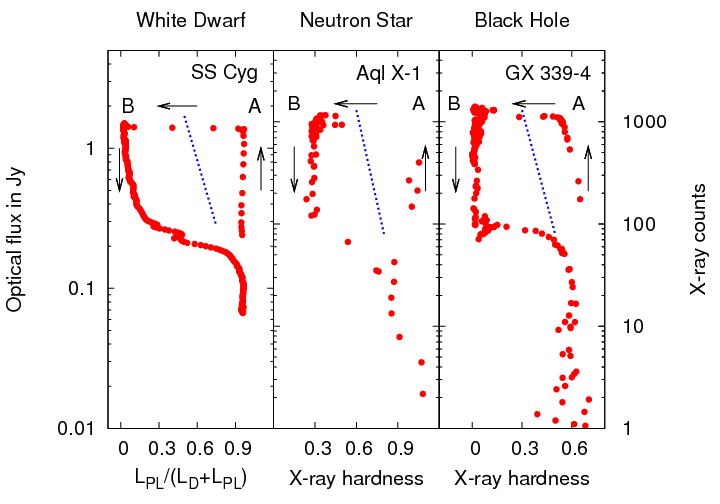
\includegraphics[width=0.7\textwidth]{figures/02-accretion/kording_hid.png}
\caption
{
{\sl Credit: Kording et al. XXXX.} 
Caption.
} 
\label{fig:kording_hid}
\end{figure}



\subsection{Jets and Outflows}


\subsection{A Global Picture}

Clearly, accretion physics is relevant to a plethora of astrophysical phenomena. 
It would also appear that the outflowing material observed in accreting systems 
has a profound effect on the accretion process itself, as well as acting 
as a spectral `filter' -- modifying, and sometimes dominating the observational 
appearance of accretion discs.